\begin{mainquestion}{rlhighpass}{RL High-Pass Filter Design}

\questionpoints
Suppose you are tasked with attenuating a 60 Hz input component signal by a factor of 100 using an RL high-pass circuit.

% =========================================================
\begin{partquestion}{attenuationdb}
{Express the attenuation factor of 100 in decibels (dB).}

\begin{answer}[0.75in]
        \[\text{Attenuation (dB)} = 20 \log_{10}(100) = 40 \text{ dB}\]
        \textit{Note: Stating the answer as a gain of $-40 \text{ dB}$ is also acceptable.}
\end{answer}

\end{partquestion}

% =========================================================
\begin{partquestion}{rolloff}
{A first-order high-pass filter has a roll-off of 20 dB/decade below the corner frequency. Using your result from (a), determine how many decades the corner frequency must be away from 60 Hz, and calculate the required corner frequency $f_c$ (in Hz) and $\omega_c$ (in rad/s).}

\begin{answer}[1.5in]
        We require 40 dB of attenuation relative to the passband (0 dB).
        Since the slope is 20 dB/decade:
        \[\text{Decades needed} = \frac{40 \text{ dB}}{20 \text{ dB/decade}} = 2 \text{ decades}\]
        
        For a high-pass filter, the attenuation occurs at frequencies *below* the corner. Therefore, the corner frequency must be 2 decades *above* 60 Hz.
        \[f_c = 60 \text{ Hz} \times 10^2 = 6000 \text{ Hz}\]
        
        Convert to angular frequency:
        \[\omega_c = 2\pi f_c = 2\pi (6000) \approx 37,700 \text{ rad/s}\]
\end{answer}

\end{partquestion}

% =========================================================
\begin{partquestion}{inductance}
{You have a $170\Omega$ resistor on hand. Given that the corner frequency for an RL circuit is $\omega_c = \frac{R}{L}$, calculate the necessary inductance value $L$.}

\begin{answer}[1in]
        From $\omega_c = R/L$, we solve for $L$:
        \[L = \frac{R}{\omega_c}\]
        
        Substitute the values ($R = 170~\Omega$, $\omega_c = 37700$ rad/s):
        \[L = \frac{170}{37700} \approx 4.509 \text{ mH}\]
        
        So, $L \approx 4.5 \text{ mH}$.
\end{answer}

    \pagebreak
\end{partquestion}

% =========================================================
\begin{partquestion}{bodeplots}
{Draw the circuit diagram for this RL high-pass filter. Then, draw the Bode plots (both magnitude and phase) of its transfer function $H(\omega)$.}

\begin{answer}[4in]
        \textbf{Circuit Diagram:}
        For an RL high-pass filter, the output is taken across the inductor.
        \begin{center}
        \begin{circuitikz}[american voltages, scale=0.8, transform shape]
            \draw (0,0) to[sV, l=$V_{in}$] (0,3)
            to[R, l=$R$] (3,3)
            to[L, l=$L$, v=$V_{out}$] (3,0) -- (0,0);
            \draw (3,3) -- (4,3);
            \draw (3,0) -- (4,0);
            \draw (4,3) to[open, v=$V_{out}$] (4,0);
        \end{circuitikz}
        \end{center}
        
        The transfer function is $H(j\omega) = \frac{j\omega L}{R + j\omega L} = \frac{j(\omega/\omega_c)}{1 + j(\omega/\omega_c)}$.
        
        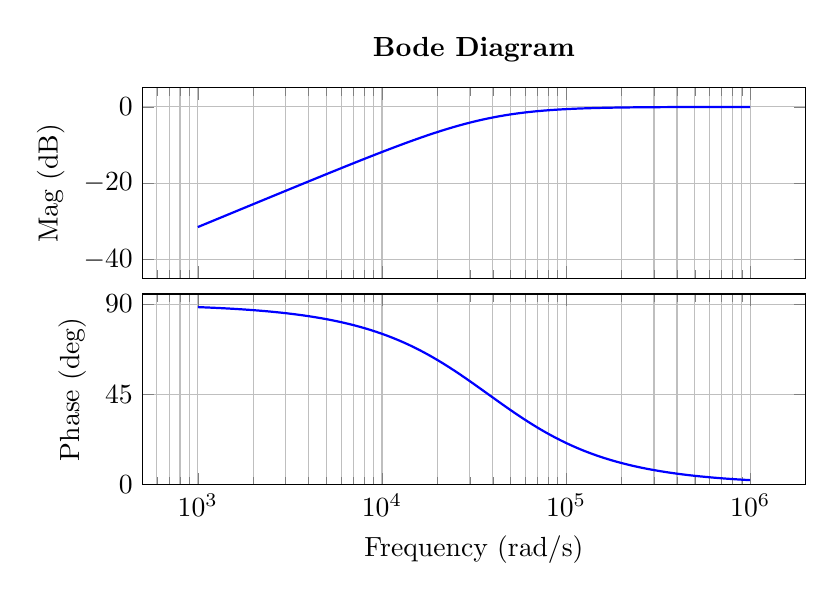
\begin{tikzpicture}
            % Magnitude Plot
            \begin{axis}[
                name=magplot,
                width=10cm, height=4cm,
                xmode=log,
                title=\textbf{Bode Diagram},
                ylabel={Mag (dB)},
                ymin=-45, ymax=5,
                grid=both,
                xticklabels=\empty
            ]
            % Mag = 20log10( wL / sqrt(R^2 + wL^2) )
            \addplot[blue, thick, domain=1e3:1e6, samples=100] {20*log10( (x*0.45) / sqrt(17000^2 + (x*0.45)^2) )};
            \end{axis}
            
            % Phase Plot - Stacked below
            \begin{axis}[
                name=phaseplot,
                at={(magplot.south west)}, anchor=north west, yshift=-0.2cm,
                width=10cm, height=4cm,
                xmode=log,
                ylabel={Phase (deg)},
                xlabel={Frequency (rad/s)},
                ymin=0, ymax=95,
                ytick={0, 45, 90},
                grid=both
            ]
            % Phase = 90 - arctan(wL/R)
            \addplot[blue, thick, domain=1e3:1e6, samples=100] {90 - atan((x*0.45)/17000)};
            \end{axis}
        \end{tikzpicture}
\end{answer}

\end{partquestion}

\end{mainquestion}
